\chapter{Background}
\label{ch:background}

\todo[Sent for review]

Git Hosting Platforms (GHPs) are online code repository platforms that are commonly used by software developers, including researchers, to host software. GitHub, GitLab, Bitbucket, and SourceForge are examples of popular GHPs. GHPs are Web-based hosting services that use and extend the functionality afforded by git, a version control system. For example, GitHub offers pages for issues, pull requests, wikis, and other additional information that is outside the scope of the git version control system but adds to the development experience. These additional pages are called ephemera and add context to the development of the repository. From a Web archiving perspective, preserving repositories hosted in GHPs is focused on preserving the Web representation of the repository within GitHub and archiving the look and feel a user would have experienced at that date and time. This approach preserves the ephemera that would not be captured with a \verb|git clone|, or retrieving copy of the code. 

To understand the importance of preserving ephemera, we will look at the GitHub repository for Keras\footnote{\url{https://github.com/keras-team/keras}}, a ``deep learning API written in Python'' and, by far, the most popular GitHub repository referenced in the corpora we studied. On June 14, 2023, we created three mementos for the Keras repository: the home page\footnote{URI-R: \url{https://github.com/keras-team/keras}}\textsuperscript{,}\footnote{URI-M: \url{https://web.archive.org/web/20230614175747/https://github.com/keras-team/keras}}, the first page of issues\footnote{URI-R: \url{https://github.com/keras-team/keras/issues}}\textsuperscript{,}\footnote{URI-M: \url{https://web.archive.org/web/20230614175841/https://github.com/keras-team/keras/issues}}, and the second page of issues\footnote{URI-R: \url{https://github.com/keras-team/keras/issues?page=2\&q=is\%3Aissue+is\%3Aopen}}\textsuperscript{,}\footnote{URI-M: \url{https://web.archive.org/web/20230614180412/https://github.com/keras-team/keras/issues?page=2\&q=is\%3Aissue+is\%3Aopen}}. After ten days, we created three more mementos\footnote{\url{https://web.archive.org/web/20230624163808/https://github.com/keras-team/keras}}\textsuperscript{,}\footnote{\url{https://web.archive.org/web/20230624163928/https://github.com/keras-team/keras/issues}}\textsuperscript{,}\footnote{\url{https://web.archive.org/web/20230624163924/https://github.com/keras-team/keras/issues?page=2\&q=is\%3Aissue+is\%3Aopen}}, one for each of the three pages we previously archived. We used the Compare tool from the Internet Archive's Wayback Machine to compare the URI-Ms for each of the three pages. 

We compared the mementos created for the Issues page and found numerous changes as shown in Figure \ref{fig:issues_compare}. In the ten days between the captures, 12 issues have been closed and 11 issues have been created, as indicated by the number of open and closed issues in Figure \ref{fig:issues_compare_1}. On the right side, we see two issues, highlighted in blue, that have been created since the capture on the left. In Figure \ref{fig:issues_compare_2}, we can see the addition new issues highlighted in blue on the right side, but we can also see that the issue highlighted in yellow on the right side has been closed since the first memento. All of these changes to the Issues page are reflecting an engaged and active development community. That is also reflected when we notice the number of comments increasing. For example, the issue titled ``AttributeError when calling model.fit() with AdamW optimizer on Apple Silicon''  on the left side has no comments, but, ten days later, the same issue now has three comments and a new tag. At the bottom of the Issues page shown in Figure \ref{fig:issues_compare_3}, we see more issues that have been closed in the ten days between captures.

\begin{figure}
    \begin{subfigure}{\textwidth}
        \centering
        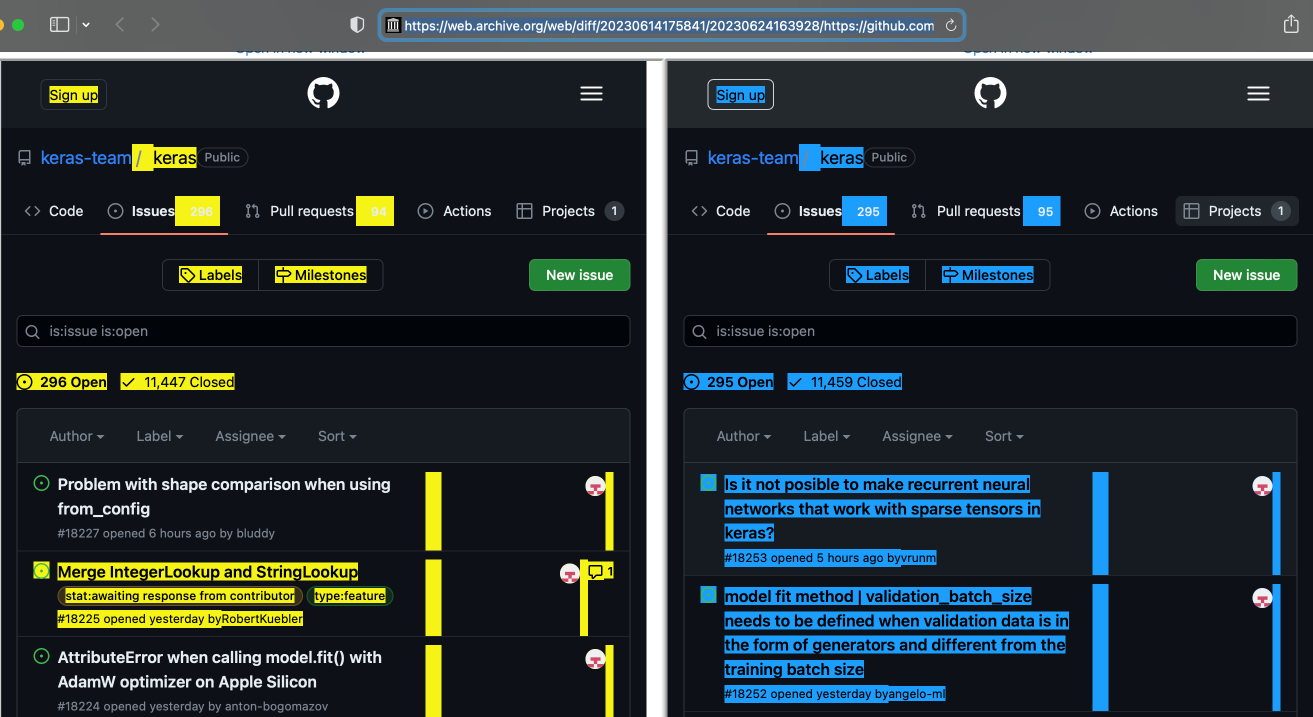
\includegraphics[ width=0.95\linewidth]{issues_compare_1.png} 
        \caption{Top of the comparison page}
        \label{fig:issues_compare_1}
    \end{subfigure}
    \begin{subfigure}{\textwidth}
        \centering
        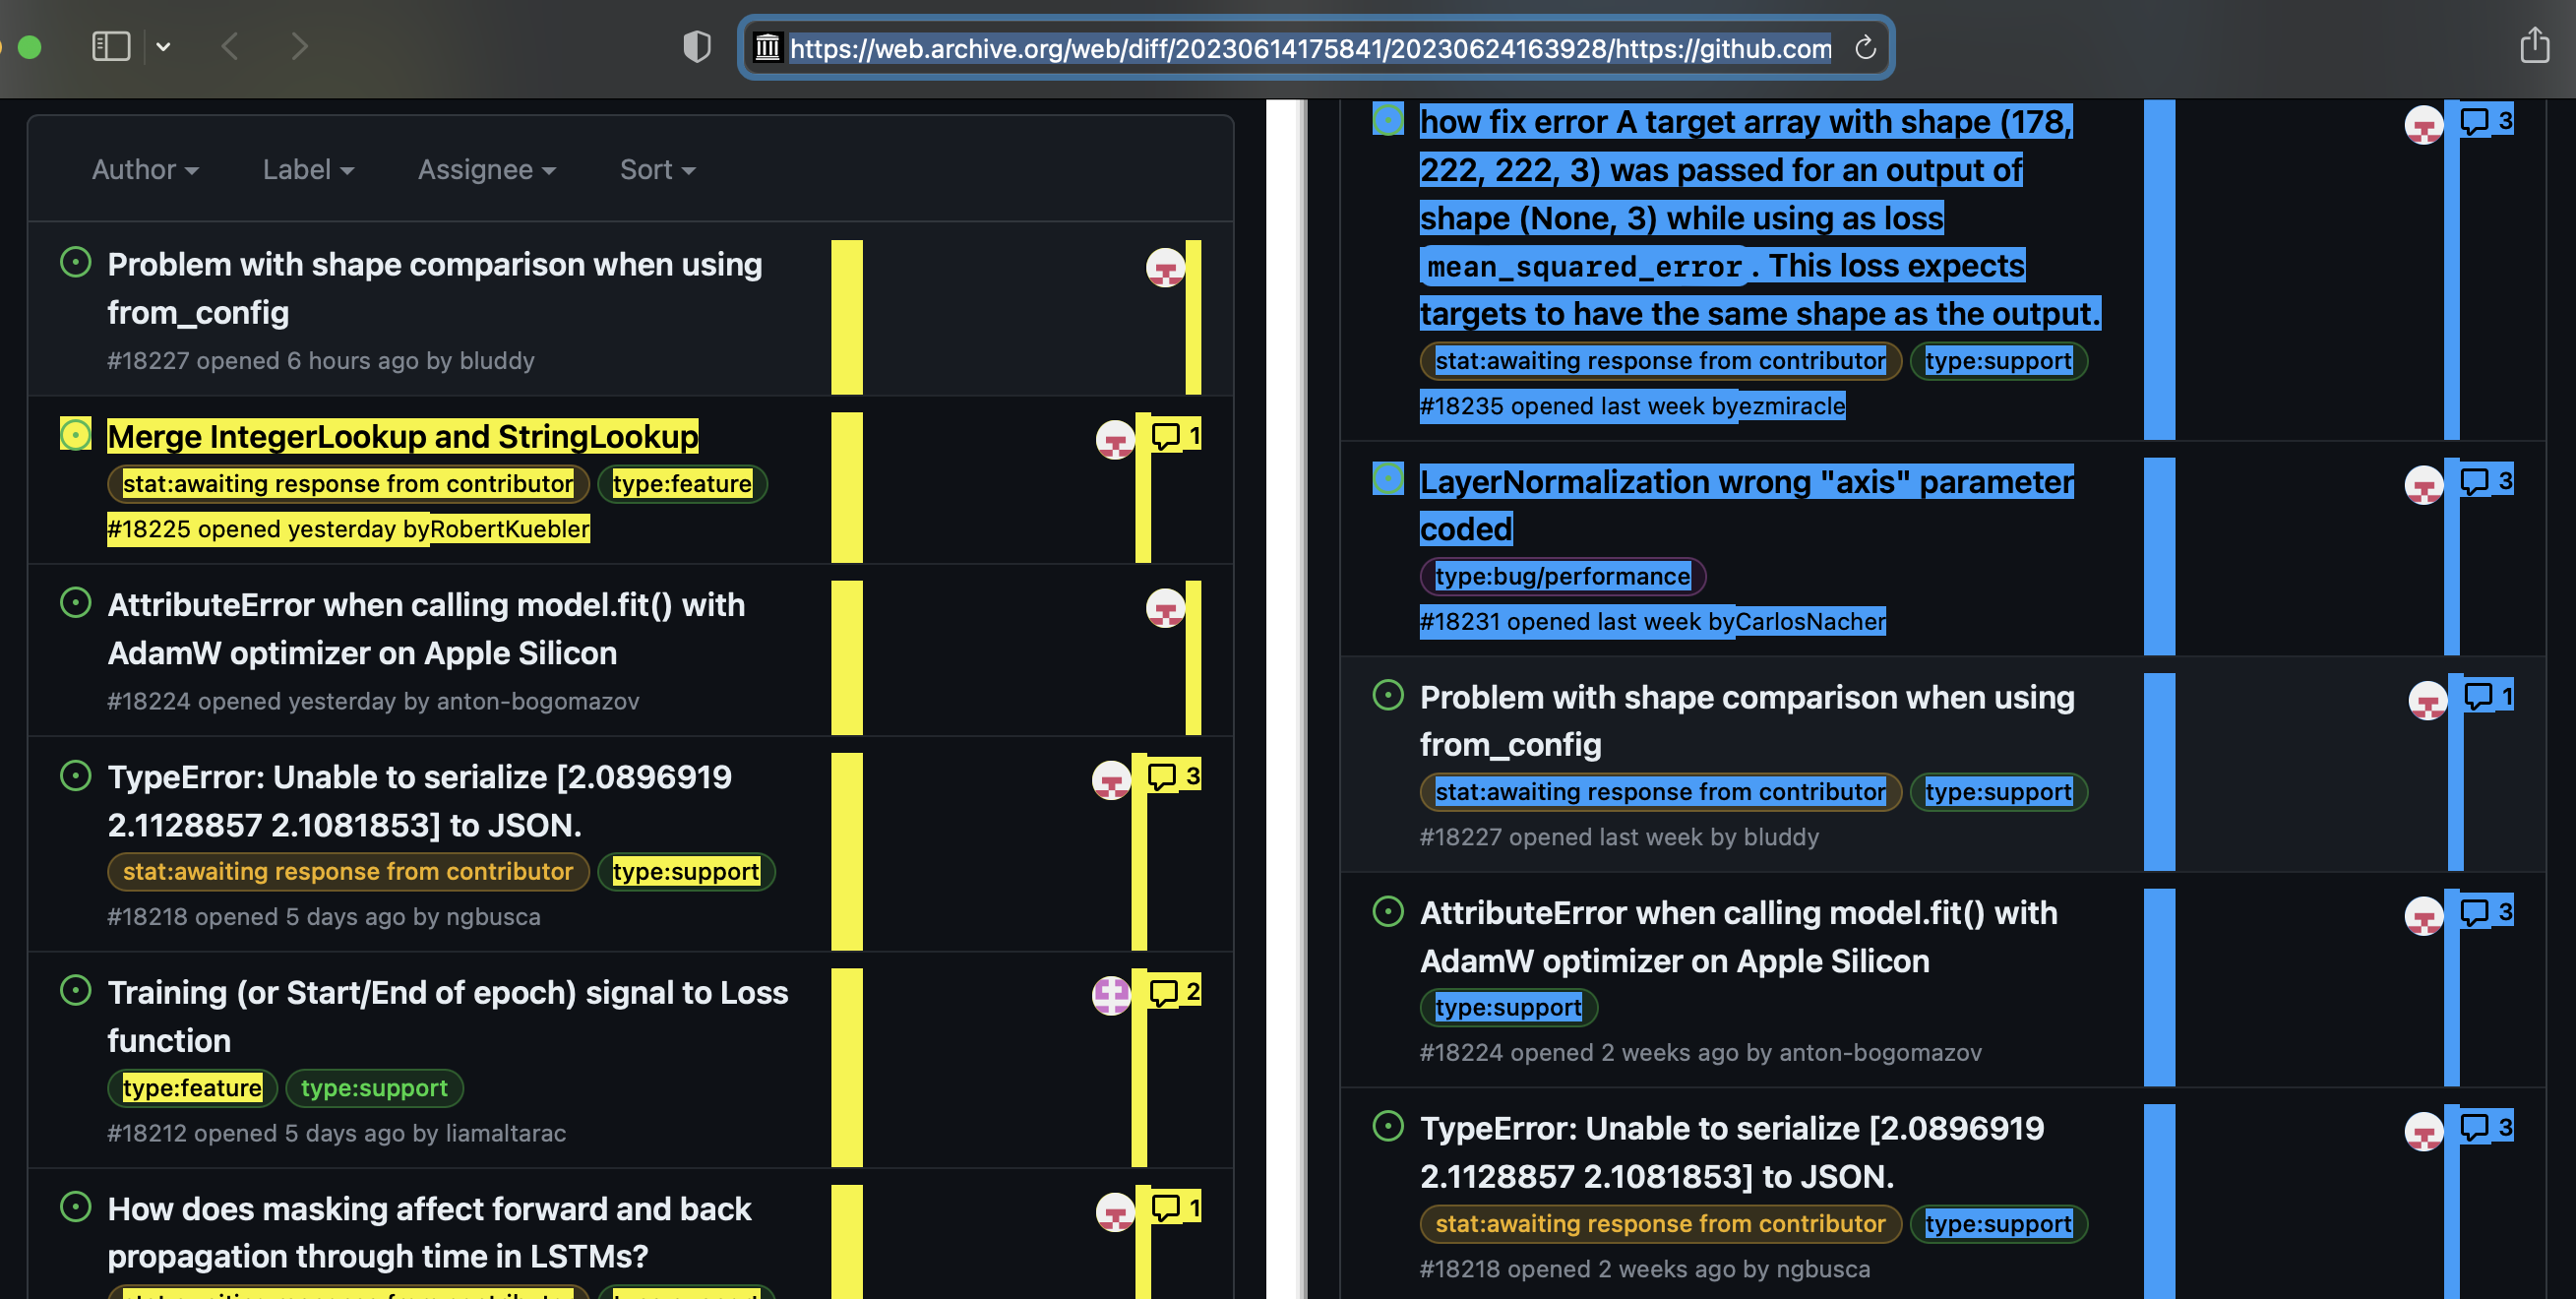
\includegraphics[ width=0.95\linewidth]{issues_compare_2.png}
        \caption{Top of the list of issues}
        \label{fig:issues_compare_2}
    \end{subfigure}
\end{figure} 

\begin{figure}
    \addtocounter{figure}{-1}
    \begin{subfigure}{\textwidth}
        \addtocounter{subfigure}{2}
        \centering
        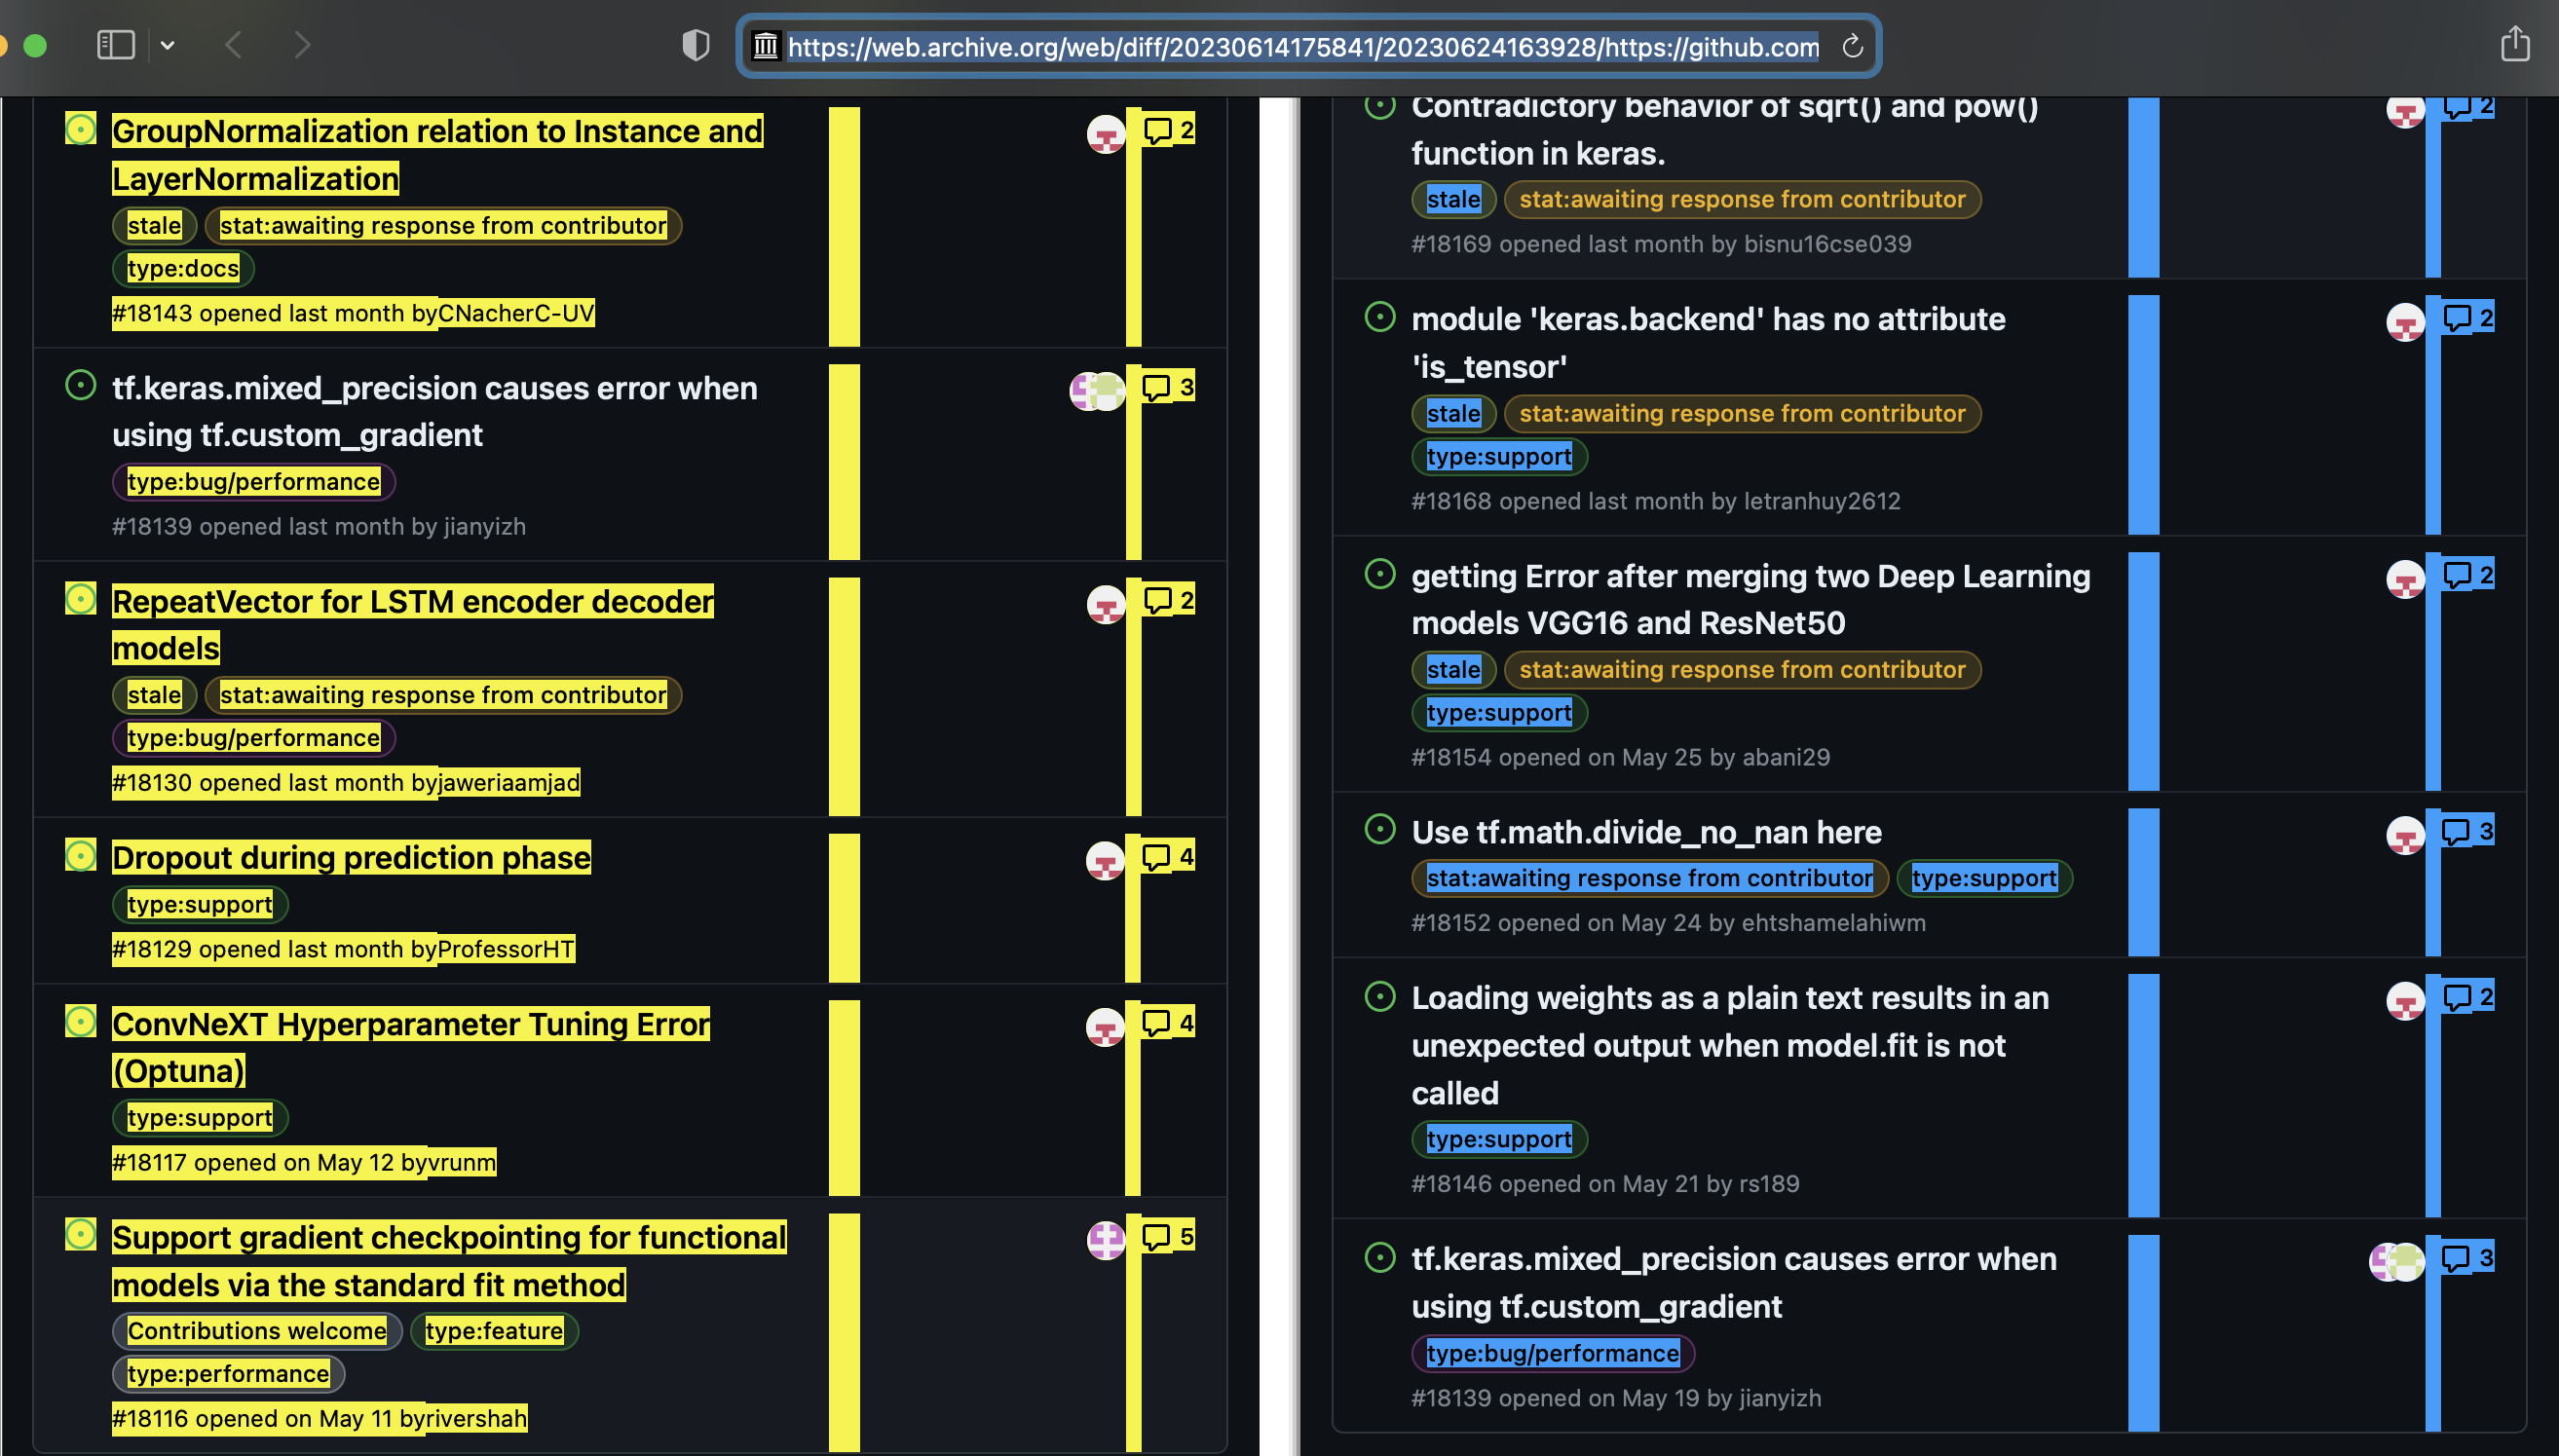
\includegraphics[ width=0.95\linewidth]{issues_compare_3.png} 
        \caption{Bottom of the comparison page}
        \label{fig:issues_compare_3}
    \end{subfigure}
    \caption[Comparing mementos of the Issues page]{Comparison of a memento of the Issues page\footnote{\url{https://github.com/keras-team/keras/issues}} from June 14, 2023\footnote{\url{https://web.archive.org/web/20230614175841/https://github.com/keras-team/keras/issues}} on the left and June 24, 2023\footnote{\url{https://web.archive.org/web/20230624163928/https://github.com/keras-team/keras/issues}} on the right}
    \label{fig:issues_compare}
\end{figure}

Despite the large number of changes reflected in the Issues page, the main repository page reflects very few changes as shown in Figure X. Changes to the commit identifier and associated commit message are the primary differences between the mementos. We found that five commits were made to the repository between the two captures, but those changes are reflected in the files themselves which are not always archived when the main repository page is archived. 



All of the commits and code changes would be preserved by archiving the code alone. However, the new and closed issues shown in Figure X would not be captured. The Issues page tells a story of the development of the code as well as the community that has created it. Users are able to ask questions, request functionality, and propose changes to be implemented in the code. Archiving the Issues page and other ephemera that surround the code provides the context for the living code product and aids in our knowledge of how the code works and why certain decisions were made. 

Internet Archive and Software Heritage are two of the primary archives that contain captures of code hosted in GHPs. Internet Archive is a Web archive and, as such, their primary goal is the preservation of the Web at large with no special emphasis on the holdings of GHPs. Web archives crawl live Web pages, or URI-Rs, and create archived versions of the live Web pages called mementos or URI-Ms. Each URI-M has an associated Memento-Datetime, the date and time that the URI-M was created. Each memento in Internet archive is uniquely identified with a combination of the URI-R and the Memento-Datetime. As a Web archive, mementos created by Internet Archive contain both the software product and the surrounding ephemera to allow users a complete picture of the hosted repository as it was available on the live Web.

Software Heritage is a non-profit organization that works to ``collect, preserve, and share all software that is publicly available in source code form'' \cite{swh-mission}. The Software Heritage (SWH) naming convention differs from the terminology defined in the Memento framework \cite{mementoprotocol}. In Software Heritage, the URI for a repository is an origin and each copy of the repository is a capture. A persistent identifier is created for each artifact within the capture, called a SWHID. While Web archives typically have a large scope covering a wide variety of content types, Software Heritage is singularly focused on the archival of source code and its development history. As a result, their captures solely archive the software product hosted in the GHP and do not archive the ephemera surrounding it. 

Scholars also deposit their code and data products in Zenodo; however, we excluded Zenodo from our study because it does not support URI searches through its Web interface or API. Users can conduct text searches or find resources through direct links, but they cannot search for a URI. 